\documentclass[12pt]{article}
\usepackage{array}
\usepackage{graphicx}
\usepackage{hyperref}

\NeedsTeXFormat{LaTeX2e}
\title{Software Engineering and Intro to Java\\Final Project\\Grade Calculation Tool}
\author{Jack Titzman} 
\date{}

\begin{document}

\maketitle 

\vspace*{10cm}
Link to Git Repository:

\href{https://github.com/jrt0799/GradeCalculator}{https://github.com/jrt0799/GradeCalculator}

\newpage

\section*{Outline}
\begin{enumerate}
	\item[1.] Title Page and Link to Git Repository
	\item[2.] Outline
	\item[3.] Vision Statement
	\item[4.] Roles
	\item[5.] Gantt Diagram
	\item[6.] Requirements
	\item[7.] Business Rules
	\item[8.] Use Cases
	\item[11.] Use Case Diagrams
	\item[12.] System Sequence Diagrams
	\item[13.] System Operations
	\item[14.] Domain Model
	\item[15.] Operation Contracts
	\item[16.] Sequence Diagrams
	\item[19.] Design Model
	\item[20.] Justification of GRASPs
	\item[21.] Use of Design Patterns
	\item[22.] Hours Spent and Logical Lines of Code
\end{enumerate}
\newpage

\section*{Vision Statement}

Many professors at Baylor University do not post their students' grades on Canvas. This forces the students to have to calculate their own grades separately. The goal of this project is to allow students to keep track of their grades without the hassle of having to calculate them themselves.

\newpage

\section*{Roles}

(Individual Project)

Project Manager - Jack Titzman

Developer - Jack Titzman

Documenter - Jack Titzman

Tester - Jack Titzman

\newpage

\section*{Gantt Diagram}

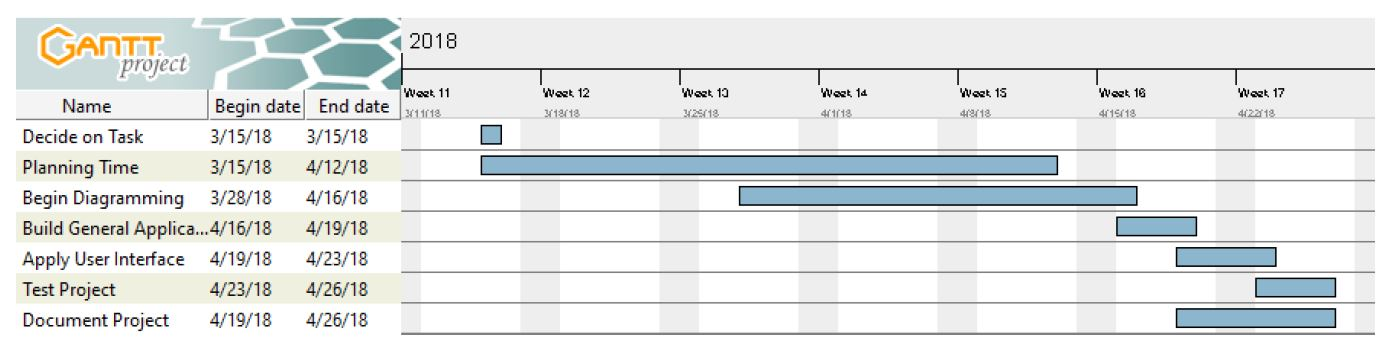
\includegraphics[width=\textwidth]{GanttDiagram}

\newpage

\section*{Requirements}

\subsection*{Functional Requirements}

\begin{itemize}
	\item User can create a new class
	\item User can remove a class
	\item User can create assignments for each class
	\item User can modify assignments for each class
	\item User can remove assignments from each class
	\item System will calculate grade for each class
	\item System will calculate GPA for each class
\end{itemize}

\subsection*{Non-Functional Requirements}

\begin{itemize}
	\item User Interface should be easy to navigate
	\item Grade calculations should be accurate
\end{itemize}

\newpage

\section*{Business Rules}

\begin{itemize}
	\item A grade of 90.0 or higher is a 4.0 GPA. A grade of 80.0-89.9 is a 3.0 GPA. A grade of 70.0-79.9 is a 2.0 GPA. A grade of 60.0-69.9 is a 1.0 GPA. A grade below 60.0 is a GPA 0.0.
	\item Assignments that are not included do not count towards the Class grade.
	\item The percentages for each assignment type in a class should add up to 100 percent.
\end{itemize}

\newpage

\section*{Use Cases}

\noindent
Use Case: Create a new class \\

\noindent
Scope: GradeCalculator application \\

\noindent
Actors: User \\

\noindent
Precondition: Application is running \\

\noindent
Postcondition: New class is added \\

\noindent
Main path:

\begin{enumerate}
	\item User starts application
	\item User chooses add new class option
	\item User fills out class details
	\item User chooses save class
	\item System creates class
	\item System adds class to application
\end{enumerate}

\noindent
Alternate paths:
\begin{enumerate}
	\item[1.] Application does not start
	\item[3.] Class details filled out incorrectly
	\item[3.1] Class creation fails
	\item[4.] User chooses cancel
	\item[4.1] Class creation fails 
	\item[5.] System fails to create class
	\item[5.1] Class creation fails
	\item[6.] System fails to add class to application
\end{enumerate}

\newpage

\noindent
Use Case: Remove a class \\

\noindent
Scope: GradeCalculator application \\

\noindent
Actors: User \\

\noindent
Precondition: class exists in application \\

\noindent
Postcondition: class is removed \\

\noindent
Main path:

\begin{enumerate}
	\item User starts application
	\item User selects a class to remove
	\item User chooses remove class
	\item System removes Class from application
\end{enumerate}

\noindent
Alternate paths:
\begin{enumerate}
	\item[1.] Application does not start
	\item[2.] No classes exist in the application
	\item[4.] System fails to remove class
\end{enumerate}

\newpage

\noindent
Use Case: Create a new assignment for a class \\

\noindent
Scope: GradeCalculator Application \\

\noindent
Actors: User \\

\noindent
Precondition: Class for assignment exists \\

\noindent
Postcondition: New assignment is added to class \\

\noindent
Main path:

\begin{enumerate}
	\item User starts application
	\item User selects a class
	\item User chooses add new assignment
	\item User enters assignment details
	\item User chooses add assignment
	\item System creates assignment
	\item System adds assignment to application
\end{enumerate}

\noindent
Alternate paths:
\begin{enumerate}
	\item[1.] Application does not start
	\item[2.] No classes exist in the application
	\item[4.] Assignment details filled out incorrectly
	\item[4.1] Assignment creation fails
	\item[5.] User chooses cancel
	\item[5.1] Assignment creation fails
	\item[6.] System fails to create assignment
	\item[7.] System fails to add assignment to application
\end{enumerate}

\newpage

\section*{Use Case Diagram}

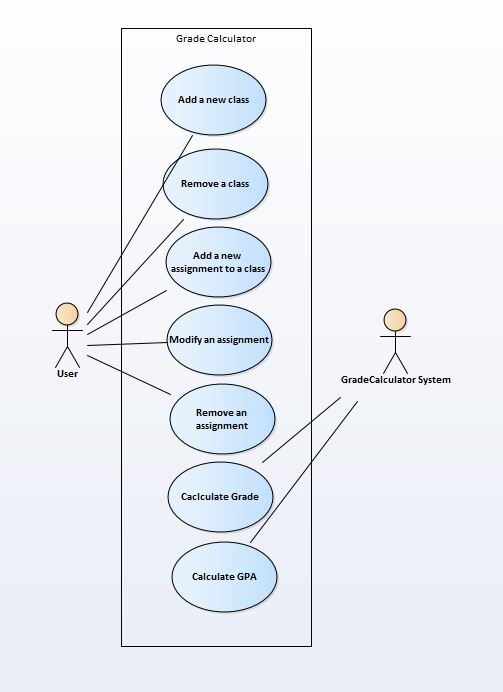
\includegraphics[width=\textwidth]{UseCaseDiagram}

\newpage

\section*{System Sequence Diagrams}

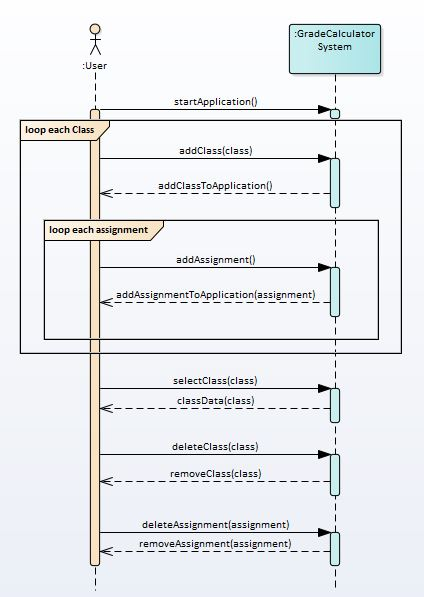
\includegraphics[width=\textwidth]{SystemSequenceDiagram}

\newpage

\section*{System Operations}

\noindent
addClassToApplication(class) \\

\noindent
addAssignmentToApplication(assignment)  \\

\noindent
classData(class) \\

\noindent
removeClass(class) \\

\noindent
removeAssignment(assignment) \\

\newpage

\section*{Domain Model}

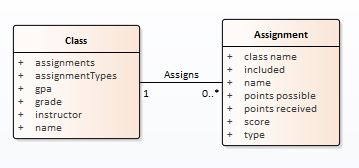
\includegraphics[width=\textwidth]{DomainModel}

\newpage

\section*{Operation Contracts}

\noindent
Operation: addClassToApplication(class)

\noindent
Cross References: Create a new class

\noindent
Preconditions:

There is a class to add to the application

\noindent
Postconditions:

The class has been added to the application \\

\noindent
Operation: addAssignmentToApplication(class)

\noindent
Cross References: Create a new assignment

\noindent
Preconditions:

There is an assignment to add to the application

\noindent
Postconditions:

The assignment has been added to the application \\ 

\noindent
Operation: classData(class)

\noindent
Cross References: Create a new class, Remove a class

\noindent
Preconditions:

There is a class in the application

\noindent
Postconditions:

The user will have the selected class' data \\

\noindent
Operation: removeClass(class)

\noindent
Cross References: Remove a class

\noindent
Preconditions:

There is a class to remove from the application

\noindent
Postconditions:

The class has been removed from the application \\

\noindent
Operation: removeAssignment(assignment)

\noindent
Cross References: Remove an assignment

\noindent
Preconditions:

There is an assignment to remove from the application

\noindent
Postconditions:

The assignment has been removed from the application \\

\newpage

\section*{Sequence Diagrams}

\noindent
Use Case: Create a new class

\noindent
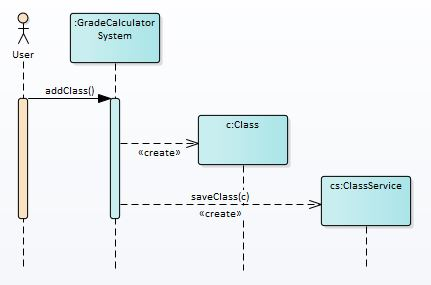
\includegraphics[width=\textwidth]{SequenceDiagram1} \\

\newpage

\noindent
Use Case: Create a new assignment

\noindent
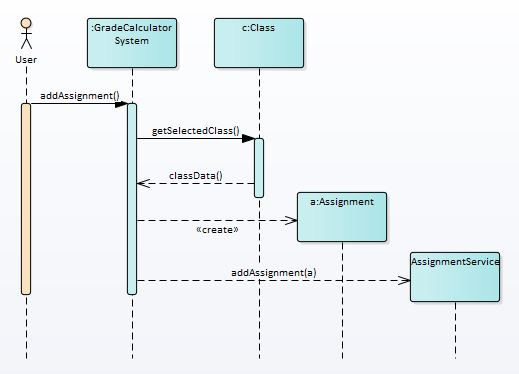
\includegraphics[width=\textwidth]{SequenceDiagram2} \\

\newpage

\noindent
Use Case: Remove a class

\noindent
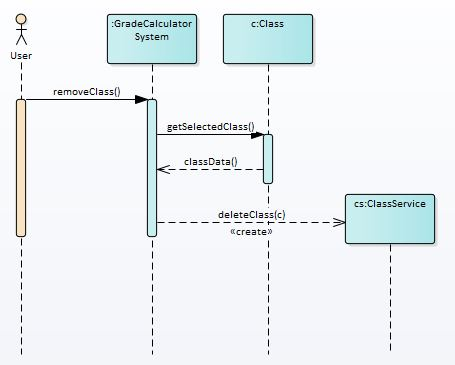
\includegraphics[width=\textwidth]{SequenceDiagram3} \\

\newpage

\section*{Design Model}

\newpage

\section*{Justification of GRASPs}

\noindent
Any time a user interacts with a component of the user interface, the ServiceResponse is used. This is using the GRASP Controller because it handles the system events.

\noindent
The classes are designed such that an AssignmentService does not know about a ClassService and vice versa. This is using the GRASP Don't talk to strangers.

\noindent
The classes are broken up into several different parts such that one element is not strongly connected to, has knowledge of, or relies upon other elements. This is using the GRASP Low Coupling.

\noindent
The classes are broken up into several different parts such that each element has strongly related and focused responsibilities. This is using the GRASP High Cohesion.

\noindent
The previous two uses of GRASPs talked about Low Coupling and High Cohesion. This was achieved by making artificial objects (ClassDAO, AssignmentDAO). This is using the GRASP Pure fabrication.

\newpage

\section*{Use of Design Patterns}

\noindent
Factory - ConnectionFactory (creates new instances of database connection) \\

\noindent
Observer - Various objects: ClassListModel, AssignmentService, ClassService, MainView (notifiesObservers when changes are made)\\

\noindent
Command - ServiceResponse from different swing components \\

\noindent
Strategy - SQLAssignmentDAO, SQLClassDAO (wraps the save, update, delete, and accessor methods including calculating grade and gpa) \\

\noindent
Proxy - Construct UI elements as placeholders and update them later. \\

\newpage

\section*{Hours Spent}

50 hours.

\section*{Logical Lines of Code}

1057

\vspace{2cm}

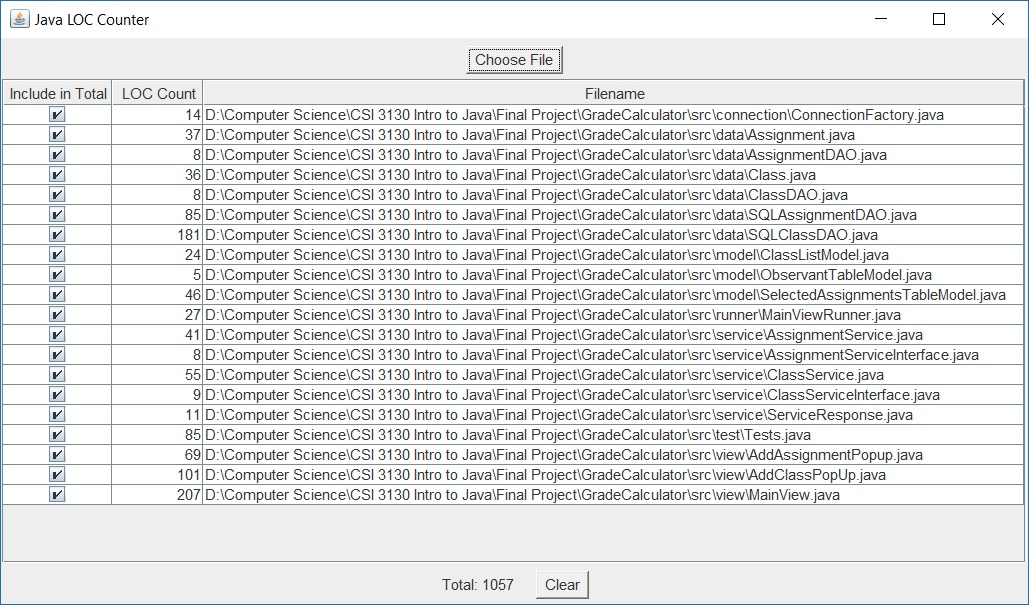
\includegraphics[width=\textwidth]{LogicalLinesOfCode}

\end{document}
